\documentclass{article}

%----------------------------------------
% Packages
%----------------------------------------
\usepackage[left=1in, right=1in, top=1in, bottom=1in]{geometry}
\usepackage{graphicx}
\usepackage{amsmath,amsbsy,amssymb,amsfonts,amsthm}
\usepackage{nicefrac}
\usepackage{mathtools}
\usepackage{color}
\usepackage{xspace} % Correct macro spacing
\usepackage[numbers]{natbib} % For citations
\usepackage{times}
\usepackage{graphicx,subfigure}
%\usepackage[small,bf]{caption}
\usepackage{algorithm,algorithmic} 
\usepackage{hyperref}

\usepackage{xcolor}
\usepackage{shadethm}

% Added for this lecture
\usepackage{parskip}
\usepackage{bbm}

\usepackage{fancyhdr}
\pagestyle{fancy}
\lhead{This is my name}
\rhead{this is page \thepage}

\usepackage{fancyhdr}
\pagestyle{fancy}
\lhead{IFT 6085 - Theoretical principles for deep learning}
\rhead{Lecture 7: January 29, 2020}


\newshadetheorem{thm}{Theorem}
\newshadetheorem{lemma}[thm]{Lemma}
\newshadetheorem{defn}[thm]{Definition}
\newshadetheorem{assm}[thm]{Assumption}
\newshadetheorem{fact}[thm]{Fact}
\newshadetheorem{prop}[thm]{Property}
\newshadetheorem{eg}[thm]{Example}


\definecolor{shadethmcolor}{HTML}{F0F0F0}
%\definecolor{shadethmcolor}{HTML}{EDEDED}
%\definecolor{shadethmcolor}{HTML}{EDF8FF}
%\definecolor{shaderulecolor}{HTML}{EDF8FF}
%\definecolor{shaderulecolor}{HTML}{45CFFF}
\setlength{\shadeboxrule}{.4pt}


\setlength\parindent{0pt}

% Packages hyperref and algorithmic misbehave sometimes.  We can fix
% this with the following command.
\newcommand{\theHalgorithm}{\arabic{algorithm}}
\DeclareMathOperator*{\argmin}{argmin}

%----------------------------------------
% Standard macros
%----------------------------------------


%----------------------------------------
% Project-specific macros
%----------------------------------------

%----------------------------------------
% Header
%----------------------------------------
\title{IFT 6085 - Lecture 7 \\ 
Elements of statistical learning theory}
\date{}

%----------------------------------------
% Document
%----------------------------------------
\begin{document} 

%----------------------------------------
% Abstract
%----------------------------------------
\maketitle

\vspace{-0.5in}
\begin{center}
This version of the notes has not yet been thoroughly checked.
Please report any bugs to the scribes or instructor.
\end{center}
\vspace{0.2in}

\textbf{Scribes}\hfill
\textbf{Instructor:} Ioannis Mitliagkas\\
\textbf{Winter 2020:} Meraj Hashemizadeh\\
\textbf{Winter 2019:} Mingde (Harry) Zhao \& Dylan Troop\\
\textbf{Winter 2018:} Brady Neal and Matthew Scicluna
\hfill


%----------------------------------------
% Body
%----------------------------------------

\newcommand{\infgc}{\inf_{g \in \mathcal{C}}}
\newcommand{\supgc}{\sup_{g \in \mathcal{C}}}

\newcommand{\Prob}{\mathbb{P}}
\newcommand{\E}{\mathbb{E}}
\newcommand{\R}{\mathbb{R}}

% Added for this lecture
\newcommand{\PP}{\mathbb{P}} %probability
\newcommand{\HH}{\mathcal{H}}   % Hypothesis class
\newcommand{\X}{\mathcal{X}}    % Input space
\newcommand{\Y}{\mathcal{Y}}    % Output space
\newcommand{\D}{\mathcal{D}}    % Data distribution
\newcommand{\yhat}{\hat{y}}     % Prediction
\newcommand{\Rhat}{\hat{R}_S}     % Empirical risk
\newcommand{\egen}{\epsilon_{\text{gen}}(h_S)}  % Generalization gap

\newcommand{\iid}{\textit{i.i.d.}}

\section{Summary}

In the previous lecture we dove into the details of Nesterov's accelerated gradient descent and made thorough comparisons with Polyak's momentum (the heavy ball method). In this lecture we will start discussing statistical learning theory, the goal of which is to determine how well a model performs on unseen data.
 
\textbf{Lecture Topics}:
\begin{itemize}
    
    \item
    Define the generalization gap and illustrate why it is the focus of our study
    
    \item 
    Introduce some concentration bounds, such as Markov's inequality, Chebyshev's inequality, Chernoff's bound and Hoeffding's Inequality
    
    \item
    Prove a bound on the generalization gap for countable, finite hypothesis classes using Hoeffding's Inequality and the Union Bound
    
    \item
    Introduce the uniform convergence framework for learning
    
    \item
    Introduce the VC dimension 
    
\end{itemize}

\section{Introduction and Notation}

The goal in machine learning is not to perform well on training data, but to perform well on unseen data. We say that a model ``generalizes well" if it performs roughly the same on test data as it does on training data. Statistical learning theory is largely concerned with theoretical bounds on this difference in performance, also known as the \emph{generalization gap}. In this lecture, we focus specifically on binary classification, but these results can be easily extended to multi-class classification.

\textbf{Notation}:
\begin{itemize}
    \item $\X$ - domain set (input space)
    
    \item $\Y$ - label set (output space)
    
    \item $m$ - number of training examples
    
    \item $S = \{(x_1, y_1), (x_2, y_2), \dots, (x_m, y_m)\}$ - training set where $(x_i, y_i) \in \X \times \Y$
    
    \item $\D$ - distribution over the data. That is, $(x_i, y_i) \sim ~ \D$. Note that in our setup we have a joint distribution rather than just $x_i$ being random and $y_i$ being a deterministic function of $x_i$
    
    \item $\HH$ - hypothesis class (class of possible models we can learn; examples below)
    
    \begin{itemize}
    
        \item $\HH_{\text{SVM}}$: class of possible SVMs on a dataset
        
        \item $\HH_{\text{LR}}$: class of possible logistic regression models on a dataset
        
        \item $\HH_{\text{NN}}$: class of possible neural networks of a fixed architecture on a dataset
        
        \item $\HH \subset \{h: \X \rightarrow \Y\}$: $\HH$ is a subset of all possible functions that map from input space to output space. Choosing this subset (hypothesis class), $\HH$, introduces inductive bias.
        
        \item In the example of binary classification on a $d$ dimensional real-valued dataset, we have $h(x_i) = \yhat_i$ where $h \in \HH, x_i \in \R^d \equiv \X, \yhat_i \in \{0, 1\} \equiv \Y$
        
    \end{itemize}
    
    \item $\ell(\yhat, y)$: loss, or error, function that measures the difference between the prediction, $\yhat$, and the true label, $y$ (e.g. 0-1 loss, squared loss, etc.)
    
    \begin{itemize}
    
        \item $\ell_{0-1}(\yhat, y) = \mathbbm{1}(\yhat \neq y)$
        
        \item $\ell_{\text{squared}}(\yhat, y) = (\yhat - y)^2$
        
    \end{itemize}
    
\end{itemize}

\section{Empirical Risk Minimization and Generalization Gap}
The goal is to identify the hypothesis $h \in \HH$ that gives the best performance on $\D$. If we knew $\D$ then we could evaluate $h$ via the risk:

\begin{defn}[True Risk]
$$R[h] \equiv \mathbb{E}_{(x,y)\sim\mathcal{D}}[l(h(x), y)]$$
\end{defn}

\begin{defn}[Empirical Risk]
$$\hat{R}_{S}[h] \equiv \frac{1}{m} \sum_{i=1}^{m}{l(h(x_i), y_i)}$$
\end{defn}


The essential task of supervised learning is to maximize the performance on all of the possible data via the adjustment of $h$ on a particularly drawn sample set $S$, which is often regarded as ``generalization''. The difference between performance of $h$ on $S$ and on $\mathcal{D}$ is the thing we want to minimize.

\begin{defn}[Generalization Gap]
Given an sample set $S = {(x_i, y_i)}$, $i \in \{1, \dots, m\}$, drawn \iid{} from $\mathcal{D}$, a hypothesis $h_S$ learnt on $S$, and a specific definition of loss $l$, the generalization gap is defined as
$$\epsilon_{\text{gen}}(h_S) = | R[h_S] - \hat{R}_{S}[h_S] |$$
\end{defn}

One of the most featured results of statistical learning theory is upper bounding this generalization gap, \textit{i.e.} to find $R(h_S) \leq \hat{R}_{S}(h_S) + \epsilon$. Modern results bound the generalization gap tighter with the help of the properties of the specific hypotheses, while the earlier results are more general which did not take into account the properties of the hypotheses. In this lecture, we will discuss the latter.

\section{Generalization Bound for Finite Hypothesis Classes}
We will first introduce some tail inequalities from probability theory and use them to bound the generalization gap for a \textbf{fixed} $h \in \HH$. Then we will use the union bound to show that the generalization gap for \textbf{any} $h \in \HH$ can be bounded.  

\begin{lemma}[Markov's Inequality]
Let $Z$ be a non-negative random variable. Then for $\forall a > 0$,
$$\mathbb{P}\{Z \geq a\} \leq \frac{\mathbb{E}[Z]}{a}$$
\end{lemma}

This may not be a tight bound, but it is useful to arrive at other results. Chebyshev's inequality is one of the most famous corollaries of Markov's inequality.

\begin{lemma}[Chebyshev's Inequality]
Let $X$ be an integrable random variable with finite expectation and finite non-zero variance. Then for $\forall a > 0$,
$$\mathbb{P}\{|X - \mathbb{E}[X]| \geq a\} \leq \frac{Var[X]}{a^2}$$
\end{lemma}

\begin{lemma}[Generic Chernoff's Bound]
Let $X$ be a random variable. Then for $\forall t > 0$ and a constant $a$,
$$\mathbb{P}\{X \geq a\} = \mathbb{P}\{e^{tX} \geq e^{ta}\} \leq \frac{\mathbb{E}[e^{tX}]}{e^{ta}}$$
\end{lemma}
The generic Chernoff's bound is a family of upper-bounds obtained by using the monotonicity of the exponential function and Markov's inequality. Note that though each $t$ gives a different bound, we can minimize the bound with respect to $t$ to get the tightest upper-bound, \textit{i.e.} $\mathbb{P}\{X \geq a\} \leq  \underset{t  \geq 0}{\inf}\,  e^{-ta} \mathbb{E}[e^{tX}] $. Such probabilistic bounds that show some random variable is close to its mean with high probability are called \emph{concentration bounds}.

\begin{lemma}[Hoeffding's Lemma]
Let $X$ be a random variable taking values in the interval $[a, b]$, with the expectation value of $0$. Then for $\forall \lambda > 0$,
$$\mathbb{E}[e^{\lambda X}] \leq e^{\frac{\lambda^2 (b - a)^2}{8}}$$
\end{lemma}
$e^{\lambda X}$ is often regarded as the moment generating function of the random variable $X$.


\begin{thm}[Hoeffding's Inequality]
Let $Z_1, \cdots, Z_m$ be independent random variables such that $\mathbb{P}\{a \leq Z_i \leq b\} = 1$ for $i = 1, \ldots, m$. Let $\bar{Z} = \frac{1}{m}\sum_{i=1}^m Z_i$. Then, for any $\epsilon > 0$:
\[
	P\left( \left| \ \bar{Z} - \E[\bar{Z}] \ \right| > \epsilon\right) \le 2 \exp\left(\frac{-2 m \epsilon^2}{(b-a)^2}\right)
\]
\end{thm}
\begin{proof}
(See Understanding Machine Learning \cite{Shalev-Shwartz:2014:UML:2621980} Appendix B.4) \\
First, we will try to shift $Z_i$ by its mean. Define $X_i \equiv Z_i - \mathbb{E}[\bar{Z}] = Z_i - \mu$, $i\in\{1, \dots, m\}$. Denote $\bar{X} \equiv \frac{1}{m}\sum_{i=1}^{m}{X_i}$.

With this we use the Chernoff bounds and get that for $\forall \lambda > 0$, % Please note that it is not \geq %2020 note: actually lambda=0  will not cause a problem
$$\mathbb{P}\{\bar{X} \geq \epsilon\} = \mathbb{P}\{e^{\lambda \bar{X}} \geq e^{\lambda \epsilon}\} \leq \frac{\mathbb{E}[e^{\lambda \bar{X}}]}{e^{\lambda \epsilon}} = e^{-\lambda \epsilon} \cdot \mathbb{E}[e^{\lambda(\frac{1}{m}\sum_{i=1}^{m}{X_i})}] = e^{-\lambda \epsilon} \prod_{i = 1}^{m}{\mathbb{E}[e^{\lambda X_i / m}]}$$
Here $X_i / m$ is a zero mean random variable that lives in the interval $[\frac{a-\mu}{m}, \frac{b-\mu}{m}]$. Thus we can use Hoeffding's lemma and get
$$\mathbb{P}\{\bar{X} \geq \epsilon\} \leq e^{-\lambda \epsilon + \frac{\lambda^2 (b-a)^2}{8m}}$$

We then minimize the RHS \textit{w.r.t.} $\lambda$ and get
$$\min_{\lambda}{e^{-\lambda \epsilon + \frac{\lambda^2 (b-a)^2}{8m}}} = \exp\left(\frac{-2m\epsilon^2}{(b-a)^2}\right)$$

By the same argument we can show that $\mathbb{P}\{-\bar{X} \geq \epsilon\} \leq e^{-\lambda \epsilon + \frac{\lambda^2 (b-a)^2}{8m}}$, and thus we get the desired result from the union of two disjoint probabilities:
\[
	P\left( | \bar{X} | > \epsilon\right) \le 2 \exp\left(\frac{-2 m \epsilon^2}{(b-a)^2}\right)
\]

\end{proof}

The expression above says that for any positive $\epsilon$, our sample mean will be at least $\epsilon$ away from its expected value with a probability that decays exponentially with the number of training examples we have.


\begin{defn}[PAC Learning]
A hypothesis class $\HH$ is (Agnostic) PAC Learnable if given some arbitrary $\epsilon, \delta > 0$ there exist an $m_\HH (\epsilon,\delta)$ such that for any $S$ with $|S| > m_\HH (\epsilon,\delta)$ we have $\egen \le \epsilon$ with probability at least $1 - \delta$. The ``probably" (\emph{P}) part of PAC corresponds to $1 - \delta$ while the ``approximately correct" (\emph{AC}) part corresponds to $\epsilon$. $m_\HH (\epsilon,\delta)$ is known as the Sample Complexity of the hypothesis class.
\end{defn}

We will now show that any finite hypothesis class $\HH$ is agnostic PAC learnable. We first derive a probabilistic bound on the following distance that holds for any $h \in \HH$:
$$\left|R[h] - \Rhat[h]\right|$$
We notice that this is just the absolute distance between the empirical average $\Rhat[h]$ and its mean since:
\begin{align*}
     \E[\Rhat[h]] = \E\left[\frac{1}{m} \sum_{i = 1}^m \ell(h(x_i), y_i)\right] = \frac{1}{m} \sum_{i = 1}^m \E[\ell(h(x_i), y_i)] = R[h]
\end{align*}


We can use Hoeffding's inequality to decide how many samples we would need to take to guarantee that  
\begin{align*}
    &P\left(\left| \ \Rhat[h] - R[h] \ \right| < \epsilon\right) > 1-\delta
\end{align*}
If we set $\delta = \exp\left(-2 m \epsilon^2\right)$ we can solve to get $m = O\left(\frac{-\log(\delta)}{\epsilon^2}\right)$. Note: this is a lower bound on the sample size which guarantees the statement above, (see \emph{Sample Complexity} in the PAC Learning definition above).

Now, suppose we consider an arbitrary $h\in\HH$ and a loss function $\ell$ with range $[0,1]$. For the random variable $\Rhat[h]$ we can use Hoeffding's inequality to get:
\begin{align*}
    P\left( \left| \ \Rhat[h] - R[h] \ \right| \ge \epsilon\right) \le 2 \exp\left(-2 m \epsilon^2\right)
\end{align*}
Note: We cannot simply replace $h$ with $h_S$ in this bound because the loss on the data points will not be independent any more, and therefore Hoeffding inequality will not hold.

So to extend this bound for $\egen$ we will use union bound:
\begin{align*}
     P\left( \left| \ \Rhat[h_S] - R[h_S] \ \right| \ge \epsilon\right) &\le P\left( \max_{h \in \HH} \left| \ \Rhat[h_S] - R[h_S] \ \right| > \epsilon\right) \\
     &= P\left( \bigcup_{h \in \HH} \left\{ \left| \ \Rhat[h] - R[h] \ \right| > \epsilon \right\} \right) \\
     &\overset{(a)}{\le} \sum_{h \in \HH}  P\left(\left| \ \Rhat[h] - R[h] \ \right| > \epsilon\right)\\
     &=2|\HH|\exp\left(-2 m \epsilon^2\right)
\end{align*}
Where (a) follows using a union bound argument. We can prove this in the case of 2 events and then use induction. In this case $P(A \cup B) = P(A) + P(B) - P(A \cap B) \le P(A) + P(B)$.

If we take $$m = O\left(\frac{\log(\frac{|\HH|}{\delta})}{\epsilon^2}\right)$$
We get the desired result:
\begin{align*}
    P\left( \left| \ \Rhat[h_S] - R[h_S] \ \right| \ge \epsilon\right) \le \delta
\end{align*}

\section{Uniform convergence}
For ERM to work, it suffices to ensure that the empirical risk of all hypothesis in $\HH$ are good approximations of their true risk. In other words, we need that uniformly over all hypothesis in $\HH$, the empirical risk is close to the true risk. In the this section we will formalize this.
\begin{defn}[$\epsilon$-representative sample]
A training set S is called $\epsilon$-representative  if:
$$
\forall h \in \HH, \,\,\, \left| \ \Rhat[h] - R[h] \ \right| \le \epsilon
$$
\end{defn}
The following lemma shows that when we have a $\frac{\epsilon}{2}$-representative sample the ERM learning rule ($h_S$) is guaranteed to be a good hypothesis.
\begin{lemma}
Assume that a training set S is $\frac{\epsilon}{2}$-representative; then, any $h_S \in \argmin_{h \in \HH} \Rhat[h]$, satisfies:
$$
R[h_S] \leq \underset{h \in \HH}{\min}\, R[h] + \epsilon
$$
\end{lemma}
\begin{proof}
$$
R[h_S] \overset{(a)}{\leq} \Rhat[h_S]  + \frac{\epsilon}{2} \overset{(b)}{\leq} \Rhat[h]  + \frac{\epsilon}{2} \overset{(a)}{\leq} R[h] + \frac{\epsilon}{2} + \frac{\epsilon}{2} = R[h] + \epsilon
$$
where $(a)$ comes from the $\epsilon$-representative definition and $(b)$ comes from the fact that $h_S$ is a ERM learning rule.
\end{proof}
This lemma shows that to be PAC learnable it suffices to prove the training set is $\epsilon$-representative with high probability.







\section{VC dimension}
In the previous parts we considered finite hypothesis classes. What happens when the number of hypotheses is infinite? We cannot just apply a union bound any more. To solve this issue, we need to have more a suitable way of measuring the “complexity” of a hypothesis class other than cardinality.
\begin{defn}[Shattering]
A set of points $S$ is shattered by a hypothesis class $\HH$ if there are hypotheses in $\HH$ that split $S$ in all of the $2^{|S|}$possible ways; i.e., all possible ways of classifying points in $S$ are achievable using concepts in $\HH$. 
\end{defn}
\begin{defn}[VC dimension of $\HH$]
The VC dimension of a hypothesis space $\HH$ is the cardinality of the largest set $S$ that can be shattered by $\HH$. If arbitrarily large finite sets can be shattered by $\HH$, then $\mathrm{VCdim}(\HH) = \infty$.
\end{defn}
Informally VC dimension is the maximum number of distinct points that a hypothesis in $\HH$ can correctly classify every possible labeling with zero error.

\textbf{Example}: (one dimensional threshold functions). Let $\mathcal{X} =  \mathbb{R}$, $\mathcal{Y} = \{0,1\}$ and $\HH = \{h_a(x) = \mathbbm{1}[x \leq a]: a \in \mathbb{R}\}$. We will try to calculate the VC-dimension of this hypothesis class. To do so we need to see how many points we can label all of its configurations using threshold functions.

\begin{figure}[ht]
\centering 
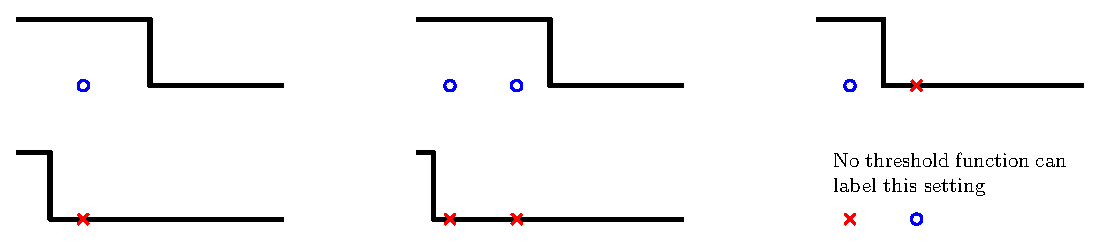
\includegraphics[width=0.98\textwidth]{vcdim.eps}
\caption{All the possible labelings for set of one and two points}
\label{fig:vcdim}
\end{figure}

As seen in Figure~\ref{fig:vcdim} our hypothesis class can label 1 points, but no set of 2 points can be labeled. Therefore the VC-dimension of this hypothesis class is 1.


%----------------------------------------
\bibliographystyle{abbrvnat}
\bibliography{Refs/lec7}
%----------------------------------------
\end{document}
